\documentclass[tikz, border=10pt]{standalone}
\usetikzlibrary{positioning, arrows.meta, shapes.geometric}

\begin{document}
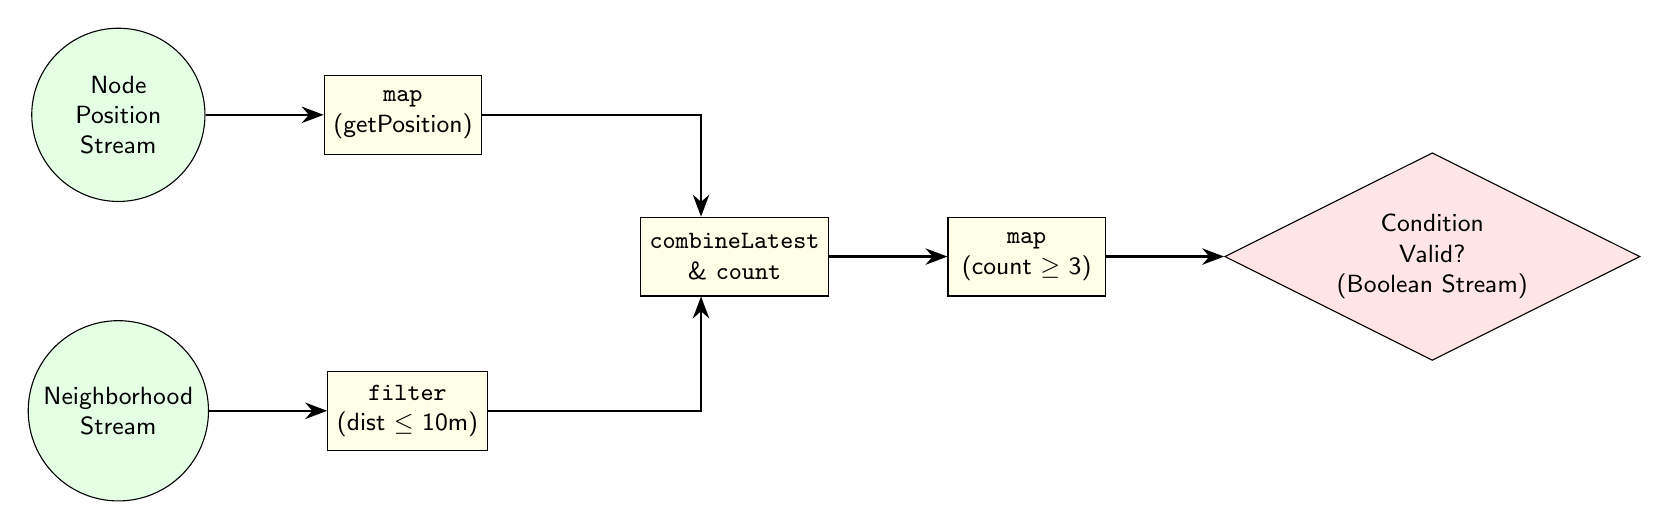
\begin{tikzpicture}[
    source/.style={draw, circle, minimum size=2.2cm, align=center, fill=green!10},
    operator/.style={draw, rectangle, minimum width=2cm, minimum height=1cm, align=center, fill=yellow!10},
    result/.style={draw, diamond, aspect=2, minimum width=3cm, minimum height=1.5cm, align=center, fill=red!10},
    arrow/.style={-{Stealth[scale=1.2]}, thick},
    font=\sffamily\small
]

% Sources
\node[source] (pos) {Node \\ Position \\ Stream};
\node[source, below=1.5cm of pos] (neigh) {Neighborhood \\ Stream};

% Operators
\node[operator, right=1.5cm of neigh] (filter) {\texttt{filter} \\ (dist $\leq$ 10m)};
\node[operator, right=1.5cm of pos] (map) {\texttt{map} \\ (getPosition)};

\node[operator, right=2cm of map, yshift=-1.8cm] (combine) {\texttt{combineLatest} \\ \& \texttt{count}};
\node[operator, right=1.5cm of combine] (cond) {\texttt{map} \\ (count $\geq$ 3)};

% Result
\node[result, right=1.5cm of cond] (final) {Condition \\ Valid? \\ (Boolean Stream)};

% Arrows
\draw[arrow] (pos.east) -- (map.west);
\draw[arrow] (neigh.east) -- (filter.west);

\draw[arrow] (map.east) -| (combine.130);
\draw[arrow] (filter.east) -| (combine.230);

\draw[arrow] (combine.east) -- (cond.west);
\draw[arrow] (cond.east) -- (final.west);

\end{tikzpicture}
\end{document}
